% !TEX encoding = UTF-8 Unicode

\documentclass[a4paper]{article}
\usepackage[utf8]{inputenc}
\usepackage{color}
\usepackage{url}
\usepackage[T2A]{fontenc} 
\usepackage[utf8]{inputenc} 
\usepackage{graphicx}
\usepackage[english,serbian]{babel}

\usepackage[unicode]{hyperref}
\hypersetup{colorlinks,citecolor=green,filecolor=green,linkcolor=blue,urlcolor=blue}


\begin{document}

\title{Skot Aronson \\
\small{Seminarski rad u okviru kursa\\Tehničko i naučno pisanje\\ Matematički fakultet}}

\author{Vidak Kozomara, Đorđe Milošević,\\Lazar Perišić, Aleksa Cvetković\\
vidak.kozomara@gmail.com, djordjem00@gmail.com,\\ lakiwow95@gmail.com, 013.aleksa@gmail.com, }

\date{oktobar 2019.}
\maketitle

\abstract{

\tableofcontents

\newpage

\section{Uvod}
\label{sec:uvod}

\textbf{Skot Džoel Aronson} (eng. \textit{Scott Joel Aaronson}) je američki teorijski informatičar i profersor informatike na Univerzitetu u Ostinu, Teksas. Njegove primarne oblasti istraživanja su mogućnosti i limiti kvantnih računara kao i računarska teorija složenosti.

\vspace{5\baselineskip}



\begin{table}[h!]
\begin{center}


\begin{tabular}{|p{10.1cm}|} \hline


\begin{center}
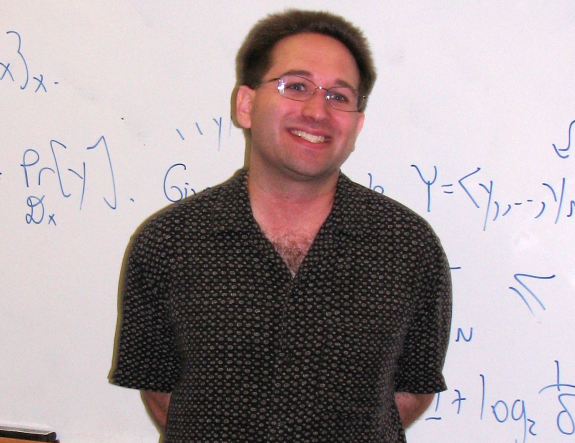
\includegraphics[scale=0.5]{Scott Aaronson.jpg}
\end{center}
\\ \hline

\end{tabular}

\hspace*{0.1cm}\begin{tabular}{|c|c|}
\textbf{Puno ime} & Skot Džoel Aronson\\ \hline
\textbf{Datum rođenja} & 21. maj 1981. \\ \hline
\textbf{Mesto rođenja} & Filadelfija, Pensilvanija\\ \hline
\textbf{Državljanstvo} & američko\\ \hline
\textbf{Zanimanje} & Teorijsko računarstvo i informatika\\ \hline
\textbf{Značajni radovi}  & "Ekvivalentnost uzorkovanja i pretraživanja"\\ \hline
\textbf{Supružnik} & Dana Moškovic\\ \hline
\textbf{Veb-sajt} & http://www.scottaaronson.com/blog/ \\ \hline

\end{tabular}
\label{tab:Slika1}

\end{center}
\end{table}

\newpage





\section{Zaključak}
\label{sec:zakljucak}



\addcontentsline{toc}{section}{Literatura}
\appendix
% \bibliography{seminarski} 
\bibliographystyle{plain}

\appendix
\section{Dodatak}



\end{document}
